\section{Introduction}
As has become clear from the discussion in the previous chapter, a crucial 
ingredient to any model of household savings is an estimate of the risk that
households are facing in the form of their income process. While traditionally
researchers have relied on a parsimonious AR(1) specification with a transitory
and a persistent shock component, which can be represented as a Markov chain 
and thus helps to ease the computational burden. Recent research has cast doubt 
on the ability of this specification to accurately capture the risk faced by 
households in the labour market though, and advances in computational 
capabilities have allowed to solve models with larger state spaces, so that 
there is a renewed interest in estimating richer statistical processes for 
household income. \vspace{1cm}
\\
\textbf{Insert discussion of recent papers based on social security data:
\citet{GKOS2015}, \citet{DHPRV2013}}

\section{A statistical model}
To inform the simulations in the following chapter, this thesis will rely on an
estimated heterogeneous income profiles (HIP) income process in the spirit of
\citet{Guvenen2009}. The process to be estimated is of the form

\begin{align}
y_{h,t}^i &= g(\theta_t, \pmb{X}_{h,t}^i) + \alpha^i + \beta^i h + z_{h,t}^i + \phi \varepsilon_{h,t}^i \label{incproc} \\ 
z_{h,t} &= \rho z_{h-1,t-1} + \pi_t \eta_{h,t}^i \label{persshock}
\end{align}

where $y_{h,t}^i$ are the log earnings of individual $i$, who has $h$ years of
labour market experience in period $t$. The function $g()$ is assumed to be 
a cubic polynomial in experience, while the individual specific parameters 
$\alpha^i$ and $\beta^i$ -- modelled as random variables with mean zero and 
variance $\sigma^2_{\alpha}$ and $\sigma^2_{\beta}$, respectively --
 capture the cross-sectional profile heterogeneity. 
$z_{h,t}^i$ is an AR(1) process with persistence $\rho$ and innovation variance
$\eta_{h,t}^i$, which captures persistent shocks to income, while
$\varepsilon_{h,t}^i$ is a purely transitory shock. Both $\eta^i$ and 
$\varepsilon^i$ are mean-zero i.i.d random variables with variances 
$\sigma^2_{\eta}$ and $\sigma^2_{\varepsilon}$, respectively. As discussed 
above, the variances of both permanent and transitory shocks have seen large
swings over the past decades, to capture this we are allowing for time-variation
in the innovation variance (denoted $\pi_t$ for the innovation to the persistent
shock component and $\varphi_t$ for the transitory counterpart). \\
To estimate the parameters of the model, an equally weighted minimum distance 
estimator is used to minimise the distance between the empirically observed 
variance-covariance structure of residual earnings (defined as $\tilde{y} \equiv 
y_{h,t}^i - g(\theta_t, \pmb{X}_{h,t}^i)$ and the variance-covariance 
structure implied by the model. In the present context, this strategy has first 
been employed by \citet{Baker98}, who estimates a very similar model to the one
 described above, although the approach has been used before for estimating 
other models in labour economics, e.g. \citet{AbowdCard89}. Our model implies 
theoretical variances and covariances given by:
\begin{align}
\var(\tilde{y}_{h,t}^i) = \underbrace{\sigma^2_{\alpha} + 2 \sigma_{\alpha \beta} h + \sigma^2_{\beta}}_{\text{contribution of profile heterogeneity}} + \var(z^i_{h,t}) + \phi_t^2 \sigma^2_{\varepsilon} \\
\cov(\tilde{y}_{h,t}^i, \tilde{y}_{h+n,t+n}^i) = \underbrace{\sigma^2_{\alpha} + 2 \sigma_{\alpha \beta} (h+n) + \sigma^2_{\beta}} + \var(z^i_{h,t}) + \phi_t^2 \sigma^2_{\varepsilon}
\end{align}
The empirical variance-covariance matrix underlying the estimation will be 
obtained by first calculating the covariance of residuals for each age-group
in a given year, and then averaging over all age groups present in a given year.
The theoretical counterpart is obtained by simply calculating the corresponding
variances and covariances from the formulas above, and forming weighted averages
over $h$ with weights corresponding to the relative frequency of age-groups in 
the empirical data. 

\section{Data}
As we are interested in the variability of our estimates, we are estimating the
process described both on PSID and BHPS data. PSID data has the advantage of 
providing a very long horizon (37 waves of data covering a total of 45 years),
which allows for the analysis of subperiods to examine changes over time. The 
BHPS, while more limited in time (18 waves of data covering 18 years) serves as
a useful comparison, while also providing excellent measures of different 
measures of household incomes pre- and post taxes and transfers, which enable us
to investigate the implications for heterogeneous income processes from 
The data is taken from all available waves of the PSID, that is years 1968 to
2013 inclusive\footnote{Note that the PSID income variable refers to income in 
the previous year, so when we talk about data from, e.g., year 1968, it is 
implied that we are referring to income in 1967.}. For our baseline estimation,
to ease comparisons, we stick to the sample selection criteria used in 
\citet{Guvenen2009}, namely:
\begin{itemize}
	\item Household heads between the ages of 20 and 64 inclusive
    \item Hourly labour earnings between \$2 and \$400 in 1993 prices
    \item Hours worked between 520 and 5110
\end{itemize}
For inclusion in our sample, an individual has to fulfil all of the above
conditions for at least 20, not necessarily consecutive, years. These sample
selection criteria leave us with 1685 individuals in our final sample
\footnote{To create the longitudinal data set from the PSID cross-sections, we
use the excellent \textit{PSIDtools} package \citep{Kohler2015}}. The main 
variable of interest in the analysis is labour income, for which we use the 
series of variables starting with \texttt{V74} in 1968\footnote{A complete list
of all variables used is available on  
\href{https://github.com/nilshg/psidJulia/blob/master/create_panel.do}{my GitHub
page}.}. Hourly earnings are taken from the variable starting with \texttt{V337}
in 1968, while hours worked are taken from the variable starting with 
\texttt{V47}. 
\begin{figure}
\includegraphics[width=\columnwidth]{BHPS_incvar}
\caption{Variance of log income and 90/10 percentile width for our sample of
BHPS households}
\label{fig:bhps_incvar}
\end{figure}

\begin{figure}
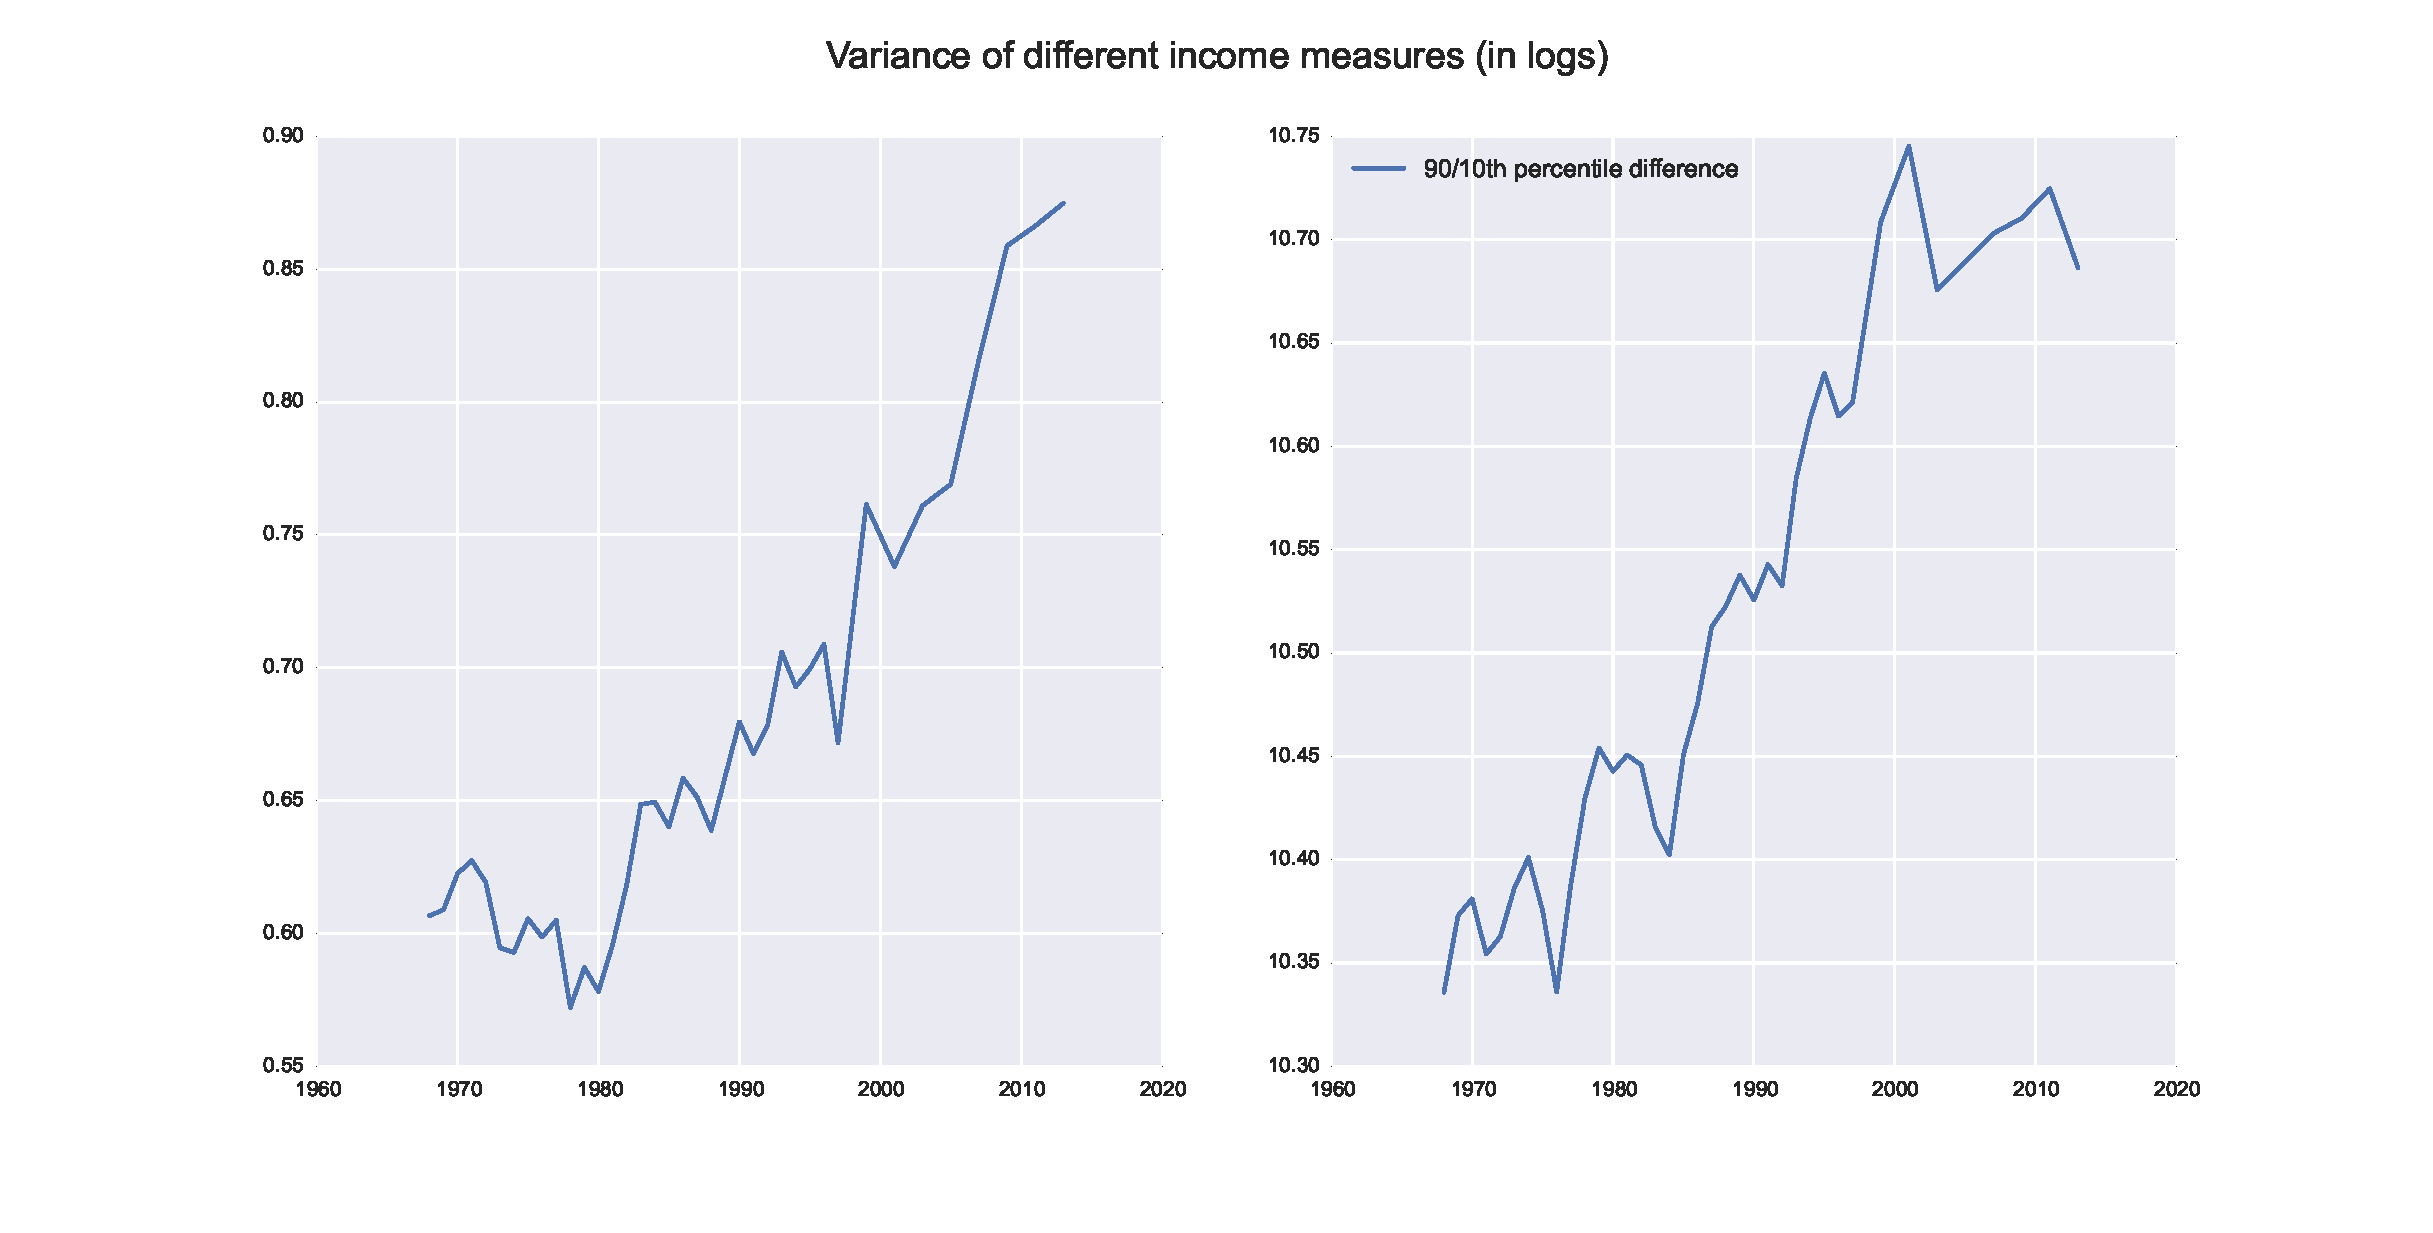
\includegraphics[width=\columnwidth]{PSID_incvar}
\caption{Variance of log income and 90/10 percentile width for our sample of
BHPS households}
\label{fig:bhps_incvar}
\end{figure}
 

\section{Results}
\begin{table}%
\begin{tabular}{l|cccccc}
                    &$\rho$ & $\sigma^2_{\eta}$&$\sigma^2_{\varepsilon}$&$\sigma^2_{\alpha}$&$\sigma^2_{\beta}$&$\sigma_{\alpha \beta}$\\
\hline
\hline \\
Guvenen (2009), RIP & 0.988 &  0.015           &   0.061                &       --          &        --        &        --             \\
Guvenen Matlab, RIP & 0.935 &  0.010           &   0.023                &       --          &        --        &        --             \\
Short sample, RIP   & 0.951 &  0.011           &   0.043                &       --          &        --        &        --             \\
Full sample, RIP    & 0.920 &  0.014           &   0.067                &       --          &        --        &        --             \\
\hline
Guvenen (2009), HIP & 0.821 &  0.029           &   0.047                &   0.022           &     0.00038      &     --0.23            \\
Guvenen Matlab, HIP & 0.853 &  0.013           &   0.030                &   0.030           &     0.00031      &     --0.30            \\
Short sample, HIP   & 0.855 &  0.017           &   0.018                &   0.022           &     0.00030      &     --0.32            \\ 
Full sample, HIP    & 0.839 &  0.017           &   0.064                &   0.047           &     0.00026      &     --0.32            \\ 
\hline
\end{tabular}
\caption{Results for the PSID sample 1968-1996; Guvenen (2009) refers to published results, Guvenen Matlab to results obtained by running
the code available on the journal website, short sample to my own estimation with the 1968-1996 data, full sample to the 1968-2013 data.}
\label{hip_rip_results}
\end{table}


